\setchapterstyle{kao}
\setchapterpreamble[u]{\margintoc}


\chapter{Event Processing and Reconstruction}
\labch{simulation_and_processing}

The analysis presented in this thesis is highly dependent on an efficient filtering and event selection to reduce the raw IceCube trigger data to a usable atmospheric neutrino sample. Based on this selection, a precise estimation of both expected SM background and expected BSM signal events can be made using MC simulations. This chapter describes the event selection chain used for state-of-the-art IceCube neutrino oscillation measurements like \sidecite{OVS_PRD}. Starting from the PMT output, both real data and simulation are processed through the in-ice trigger, the online filter and processing, and the low-energy event selection to produce a neutrino dominated sample. Once the sample is small enough for more sophisticated reconstruction techniques to be feasible to run, the events can be reconstructed with the existing IceCube reconstruction algorithms. Using the reconstruction outputs and some high level variables that are also computed, the final event selection is performed. \todo{re work with combined reco and so on? (RED)}


\section{Processing} \labsec{processing_chain}

After the detector simulation is performed, all MC and data are processed in exactly the same way. This section explains the trigger and event selection that is applied starting from the raw voltage measured by the PMTs. It is split in different steps run inside the ice, at the South Pole, and after the data was transferred to the North. The complexity and computational cost of the processing increases with each step, while the total number of events reduces, making it feasible and reducing the use of computational resources on events that are not of interest for the analysis. 


\subsection{Trigger and Filter} \labsec{trigger_and_filter}

Before the data can be sent to the North, the initial signal coming from the PMT is a voltage waveform that has to be digitized (for data) and then information of photon hits has to be extracted (also for the MC coming from the detector response simulation). The trigger and filter explained here are tailored to select events that passed through the DeepCore volume, while rejecting background events (either from atmospheric muons or from random noise). There are other filters used in IceCube which will not be explained here, since they are not relevant for this work. A full description of the instrumentation and the online systems can be found in \sidecite{Aartsen:2016nxy}.


\subsubsection{In-ice Trigger} \labsec{trigger}

\todo{Include some low level plots like the trigger efficiency for the HNL simulation (ORANGE)}

\begin{marginfigure}
    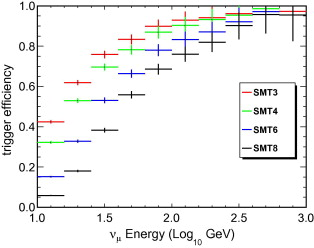
\includegraphics{figures/simulation_and_processing/trigger/trigger_efficiency.jpg}
	\caption[IceCube trigger efficiencies]{Efficiencies of different IceCube and DeepCore triggers, taken from \cite{DeepCore_design_Abbasi2012615}.}
    \labfig{trigger_efficiencies}
\end{marginfigure}

The trigger is applied inside the DOM in the ice before sending the information to the ICL on the surface. The time dependent voltage curves are captured if a pre-defined threshold value is exceeded. Once the threshold set to the equivalent of \SI{0.25}{PE} is crossed, \SI{6.4}{\micro\second} of the waveform are coarsely digitized by a \textit{Fast Analog-to-Digital Converter (FADC)} with a sampling rate of \SI{40}{\mega\hertz}. Additionally, the first \SI{427}{\nano\second} are digitized using an \textit{Analog Transient Waveform Recorder (ATWD)} with a sampling rate of \SI{300}{\mega\hertz} \sidecite{ABBASI2009294_data_acquisition}, but only if some trigger condition is met, because this readout frequency is too high to be sampled directly and requires some buffering. For DeepCore, the HLC condition already mentioned in \refsec{ice_and_DOMs} has to be met for three DOMs inside the fiducial volume within a time window of \SI{5}{\micro\second}. If this is the case, all waveforms that crossed the threshold within a \SI{20}{\micro\second} time window around the trigger are digitized and sent to the ICL for further processing. This trigger is called \textit{Simple Multiplicity Trigger 3 (SMT-3)}. The DOM hits that are read out in this process, but do not meet the HLC condition, are called \textit{soft local coincidence (SLC)} hits. The rate of the DeepCore SMT-3 trigger is $\sim$\SI{250}{\hertz} \sidecite{2017JInst..12P3012A_Instrumentation_Systems}, accepting $\sim$\SI{70}{\percent} of $\nu_\mu$-CC events at \SI{10}{\gev} and $\sim$\SI{90}{\percent} at \SI{100}{\gev} \sidecite{DeepCore_design_Abbasi2012615}. The trigger efficiencies for different SMT triggers, including the DeepCore SMT-3, are shown in \reffig{trigger_efficiencies}.


\subsubsection{Online Filter} \labsec{online_filter}

The digitized waveforms are sent to the ICL, where a further filter is applied \textit{online}\sidenote{Where \textit{online} means running on hardware at the South Pole.}. First, the WaveDeform algorithm is run to extract photon arrival times and charge from the waveforms, then the DeepCore filter is applied, which is an iterative hit cleaning starting from HLC hits and removing any hits outside a \SI{125}{\meter} radius and a \SI{500}{\nano\second} time window (called \textit{radius-time cleaning (RT-cleaning)}) of the initial hit. This mainly rejects unphysical SLC hits, which are potentially caused by random noise. The following selection steps are done using the resulting cleaned pulses.

Next, an additional cut is applied to reject events that are likely to be caused by atmospheric muons. This is done by splitting the hits depending on whether they were inside the DeepCore fiducial volume or outside and then calculating the speed of each hit outside the fiducial volume towards the \textit{center of gravity (COG)} of the hits inside. If one of them has a speed close to the speed of light, the whole event is rejected, because this is a strong indication for a muon event.

As input for the further selection levels, a few event properties, like vertex position and direction, are determined using fast and simple event reconstructions. After the DeepCore online filter, the rate is about \SI{15}{\hertz}, which can be sent to the North via satellite for further processing.


\subsection{Event Selection} \labsec{event_selection}

After the data was sent to the North, the \textit{offline} filters and selection are applied to further recude reduce the background of atmospheric muons and noise. The selection is split into three levels referred to as \textit{Level 3-5 (L3-L5)}, which bring down the neutrino and muon rate to $\sim$\SI{1}{\milli\hertz}, while the remaining fraction of random noise is below \SI{1}{\percent}.


\subsubsection{Level 3} \labsec{level_3}

At the first offline filtering level, Level 3, 1D cuts are used to reduce atmospheric muons, pure noise, and coincident muons. These cuts are targeting regions where the data/MC agreement is poor, so that more sophisticated \textit{machine learning (ML)} techniques can be applied at later levels. The cuts are made using 12 control variables, that are inexpensive to compute for the very large sample at this stage. The variables are related to position, time, and overall number of hits in the event.

Pure noise hits, that are temporally uncorrelated, are cleaned by applying a \SI{300}{\nano\second} sliding window, requiring the containment of more than 2 hits at its maximum. Additionally, an algorithm is run to check whether the hits show some directionality, accepting them only if they do.

To reduce the amount of muons a series of cuts is applied using spatial and temporal information. Events that have more than 9 hits observed above \SI{-200}{\meter} or the first HLC hit above \SI{-120}{\meter} are rejected as well as events where the fraction of hits in the first \SI{600}{\nano\second} of the event is above 0.37, ignoring the first two hit DOMs. Additionally, the ratio between hits in the veto region and the DeepCore fiducial volume is required to be below 1.5.

If a muon enters the detector after the data acquisition was already triggered, it causes events that span over a much larger time range. To reduce those coincident events, the time difference between first and last pulse cannot be above \SI{5000}{\nano\second}. This cut mainly affects a region of very poor data to MC agreement, because coincident events are not simulated at all.

The L3 cuts remove \SI{95}{\percent} of the atmospheric muons and >\SI{99}{\percent} of pure noise hits, while keeping >\SI{60}{\percent} of the neutrino events. The sample now roughly contains muons/neutrinos/noise at a ratio of 100:10:1 with a total rate of $\sim$\SI{0.5}{\hertz}.

\todo{add example plots (2?) for L3 cut variables and applied cuts (YELLOW)}

\subsubsection{Level 4} \labsec{level_4}

After the total rate was reduced by the simple cuts of L3 and the overall agreement between data and MC is established, ML techniques can be applied to further reduce the background. For Level 4, two \textit{Boosted Decision Trees (BDTs)} \sidecite{BDT} classifier are trained to separate neutrino events from atmospheric muons and noise hits, separately. The output of each classifier, a probability score, can be seen in \reffig{level_4_classifiers}. The noise filter is applied first and an event passes the score if it is larger than 0.7, reducing the noise hits by a factor of 100, while keeping \SI{96}{\percent} of neutrinos. Then the second BDT classifier is applied to reject muons. It was trained partly on unfiltered data, which consists of >\SI{99}{\percent} atmospheric muons, to reject the data and keeping the neutrinos from the simulation. Rejecting events with a score smaller than 0.65 removes \SI{94}{\percent} of atmospheric muons while keeping \SI{87}{\percent} of neutrinos. This fraction varies depending on the flavor and interaction type, $\nu_\mu$-CC events for example, which have a muon in the final state, are therefore reduced to \SI{82.5}{\percent}. After applying the L4 cuts based on the BDT classifier outputs, the sample is still dominated by atmospheric muons, while the noise rate dropped to below most neutrino types.

\begin{figure*}
\centering 
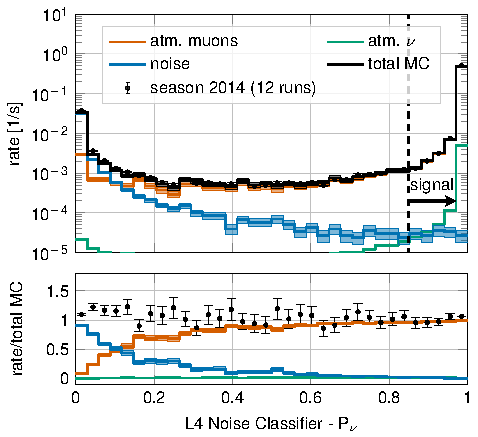
\includegraphics[width=0.49\linewidth]{figures/simulation_and_processing/selection/l4_noise_classifier_probnu.pdf}
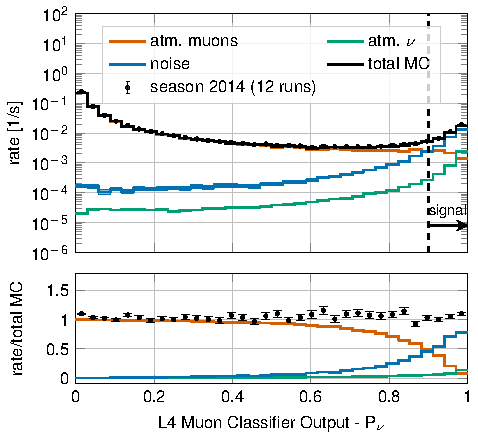
\includegraphics[width=0.49\linewidth]{figures/simulation_and_processing/selection/l4_muon_classifier_probnu.pdf}

\caption[Level 4 classifier outputs (muon and noise)]{Distributions of Level 4 noise classifier output (left) and muon classifier output (right), where larger values indicate more neutrino-like and lower values more noise-like/muon-like. Taken from \cite{OVS_PRD}.}
\labfig{level_4_classifiers}
\end{figure*}


\subsubsection{Level 5} \labsec{level_5}

Level 5 is the final selection level, before event reconstructions are applied. This level aims to reduce the remaining atmospheric muon rate below the rate of neutrinos. Muons not rejected by the earlier levels are those that produced little or no light in the veto regions. One possible reason is that they passed through one of the un-instrumented regions between the strings \todo{add some figure showing the corridors? (YELLOW)} called \textit{corridors}. To reject those, special corridor cuts, based on the number of hits they produced close to a potential corridor they passed through. The potential corridor in questions is identified based on a simple infinite track fit. In addition to the corridor cuts, starting containment cuts are applied to reject events that start at the edge of the fiducial volume. Events with more than seven hits in the outermost strings of the detector or those that have a down going direction in the uppermost region are rejected. This further reduces the fraction of muons by \SI{96}{\percent} while keeping \SI{48}{\percent} of neutrinos. The rates after this level are \SI{1}{\milli\hertz} and \SI{2}{\milli\hertz} for neutrinos and muons, respectively, making it a neutrino dominated sample.

\todo{add table with rates per level (split in flavor) - maybe better in analysis chapter to also show signal? (RED)}


\section{Reconstruction} \labsec{reconstruction}

% Several methods exist to reconstruct events at the energies relevant for this work (\SIrange{10}{100}{\gev}).
In the energy range most relevant for this work, between \SIrange[range-phrase={~and~}]{10}{100}{\gev}, the light deposition is very low and only a few DOMs detect light, making the reconstructions difficult. In \sidecite{low_energy_reco_IC} two classical methods are described, which have partly been applied in one recent IceCube atmospheric neutrino oscillation measurement using a
% golden\sidenote{The golden sub-sample only uses events that have direct photon hits.} 
sub-sample of the DeepCore sample \sidecite{OVS_PRD}. The algorithm used in this work on the other hand, is a newer method that applies a \textit{convolutional neural network (CNN)} to reconstruct the events and determine some discriminating quantities. The latest muon neutrino disappearance result from IceCube \sidecite{flercnn_analysis_result} is based on this reconstruction.


\subsection{Fast Low-Energy Reconstruction using Convolutional Neural Networks} \labsec{flercnn_reconstruction}

As the name \textit{Fast Low-Energy Reconstruction using Convolutional Neural Networks (FLERCNN)} already indicates, the FLERCNN reconstruction \sidecite{flercnn_proceedings, flercnn} is a CNN optimized to reconstruct IceCube events at low energies ($<$\SI{100}{\gev}) in a fast and efficient manner, by leveraging the approximate translational invariance of event patterns within the detector.
% The network is trained to find the connection between the hit pattern and the events properties by identifying patterns similar to how CNNs are applied effectively in image classification.\todo{add references for CNN image classification?} The patterns are an imprint of the neutrino interactions that can happen anywhere in the detector, which should result in translational invariance of the events. CNNs were shown to have very good performance in identifying patterns in images, independent of their location. By combining several layers of filters of different dimensions, a map of spatial features is created from the input data and more complex features can be reconstructed.
The architecture of the network is very similar to the preexisting IceCube CNN event reconstruction \sidecite{dnn_reco_mirco}, but optimized on low-energy events and specifically tailored to include the DeepCore sub-array. Only the eight DeepCore strings and the central 19 IceCube strings are used for the reconstruction (compare to \reffig{icecube_top_view}). Because of the different z-positions of the DeepCore and IceCube DOMs, they are divided into two networks that are combined in the final layer of the network. The full architecture is shown in \reffig{flercnn_network_structure}. The first dimension of the network is the string index, while the second dimension is the order of the DOMs along the vertical axis. The horizontal position of the DOMs is not used, since the strings are arranged in an irregular pattern. The information from the DOM hits is summarized into five charge and time variables, which make up the last dimension of the input layer. The variables are the total summed charge, the time of the first hit, the charge weighted mean time of the hits, the time of the last hit, and the charge weighted standard deviation of the hit times.

\todo{add image with selected strings used for flercnn IC and DC (YELLOW)}

\begin{figure}
    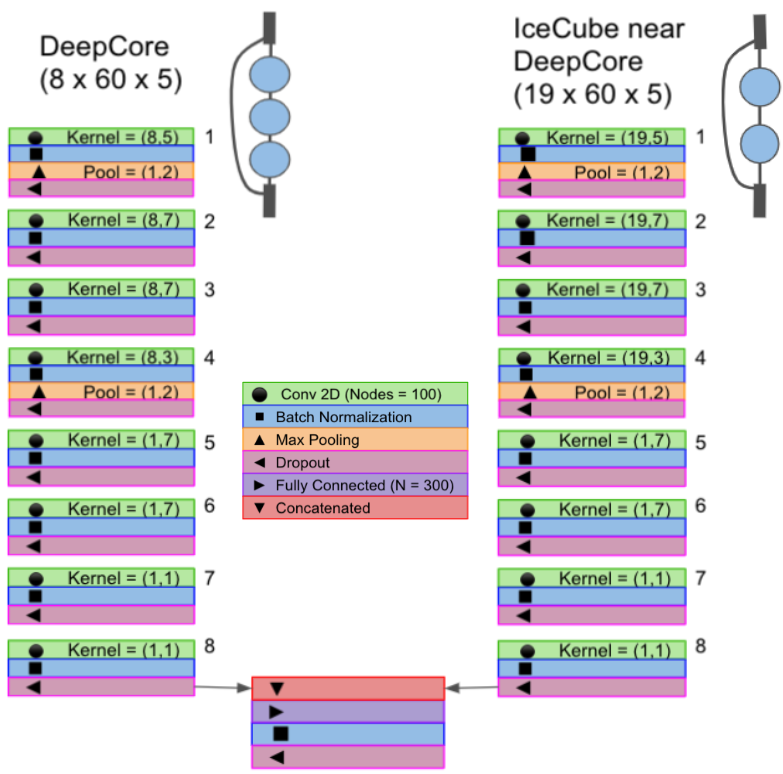
\includegraphics{figures/simulation_and_processing/flercnn/Detailed_CNN_Architecture_combined.png}
	\caption[FLERCNN architecture]{Architecture of the FLERCNN neural networks, taken from \cite{flercnn_proceedings}.}
    \labfig{flercnn_network_structure}
\end{figure}


Five different networks are trained using this architecture. Three networks do the regression of the events' energy, zenith angle, and the starting vertex ($x,y,z$ position), while two of them are used for classification. One is trained to predict the probability of the event being a track (used as PID) and the other to predict the probability of the event being a muon. Each network is trained with an MC sample modified to have a flat distribution in the target variable, to be unbiased for that variable and ideally extending outside the target reconstruction region.
% Additionally, the activation function and the loss function are adapted, according to the wanted output of the network.
For the classification tasks the loss function is the \textit{binary cross entropy} and the activation function is a \textit{sigmoid}. To perform the regression of zenith and vertex position, the loss function is the \textit{mean squared error (MSE)}, while for the energy it is the \textit{mean absolute percentage error}. The activation for all regression tasks is \textit{linear}.

\todo{add some performance plots of the FLERCNN reconstruction (ORANGE)}

\todo{There is more information on pre-processing the samples and preparing the input features, and training each cnn, but I'm not sure if that might be too much detail? (YELLOW)}

% \textit{INFO on resolutions:} Note that all analysis cuts are included in these resolution calculations, which results in an artificial resolution decrease near $E_{true} \approx 100$ GeV in Figure \ref{fig:EnergyResolution} due to the cut at $E_{reco} < 100$ GeV.


\subsection{Analysis Selection} \labsec{analysis_cuts}

Before the reconstruction is applied a few additional high level variables are computed, which are from fast and inexpensive algorithms. Then the reconstruction is performed by applying the trained FLERCNN networks to get the output quantities. After that, another BDT classifier is trained to further reduce the muon background for the final sample. The BDT is trained on five high level variables, where three are FLERCNN reconstruction variables (vertex $z$, $\rho_{36}$\sidenote{A radial variable that is often used in IceCube, is the horizontal distance to string 36 called $\rho_{36}$, which is basically the distance to the center of IceCube.}, and muon probability) and two are lower level variables (L4 muon classifier output and L5 corridor cut variable). To train the BDT, the FLERCNN nominal simulation set is used, only using events with $\cos(\theta_{zenith})\leq 0.3$. The output of the BDT is the neutrino probability and a cut at 0.8 is applied to reject events with a high probability of being a muon. \reffig{muon_bdt_id} shows the output of the BDT classifier, where the neutrinos in both training and testing sets are gathered at 1 and muons are around 0, which shows great classification power.

\begin{figure*}
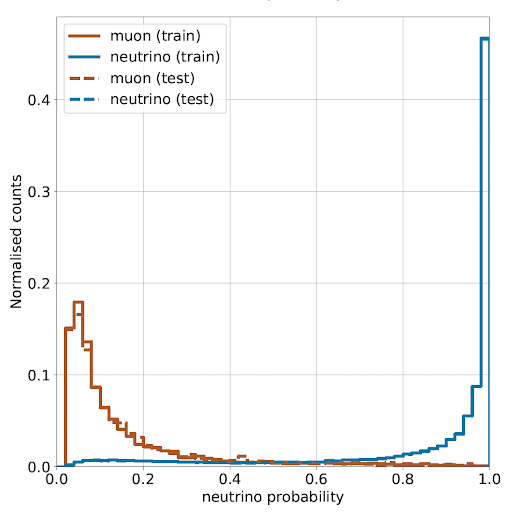
\includegraphics[width=0.49\linewidth]{figures/simulation_and_processing/flercnn/flercnn_muon_classifier.png}
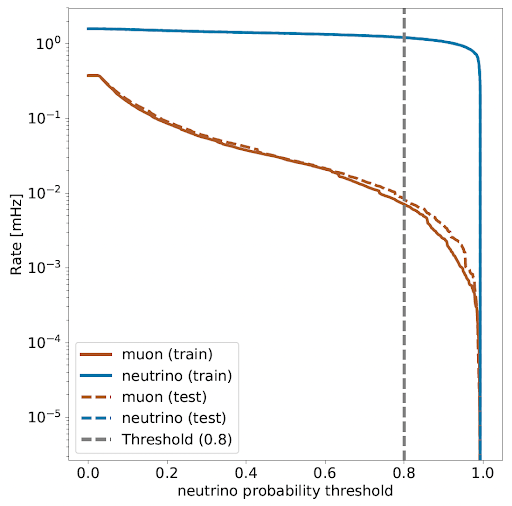
\includegraphics[width=0.49\linewidth]{figures/simulation_and_processing/flercnn/flercnn_muon_classifier_rate_vs_threshold.png}
\caption[FLERCNN muon classifier probability distributions]{FLERCNN muon classifier output score (left) and rate of neutrinos and muons as function of muon classifier cut (right). Taken from \cite{flercnn_analysis_internal_note}}
\labfig{muon_bdt_id}
\end{figure*}

\todo{add reference for flercnn analysis internal note (ORANGE)}

To get the final, pure sample of well reconstructed neutrinos another set of cuts is applied. The first cuts are meant to reject events with poor reconstruction quality, by requiring the events to fall into the DeepCore volume, where the denser, better instrumented detector leads to enhanced resolution. The cuts are applied on the vertex $z$ and $\rho_{36}$ and are listed in \reftab{analysis_cuts}. The FLERCNN reconstruction was optimized for atmospheric neutrino analyses which are mainly in the region below \SI{100}{\gev} and there are very few events with energies below \SI{5}{\gev}, so the reconstructed energy is required to be in that range. Additionally, rejecting events with fewer than seven hits in the selected DOMs used for FLERCNN showed to increase the resolution.

Another set of cuts is applied to make sure the agreement between data and MC is good. To remove coincident muon and neutrino events, cuts are applied to the number of hits in the top 15 layers of IceCube DOMs and the number of hits in the outermost IceCube strings. Coincident random noise events are removed by requiring more than three hit DOMs from direct photons\sidenote{\textit{Direct photons} are photons that were not scattered on their way from the interaction vertex to the DOM.}. Neither of the two coincident event types are simulated, which can be seen as bad agreement between data and MC. The last cut is on the reconstructed cosine zenith, which is required to be smaller than 0.04 to reject down-going muons.

\begin{table}
    \small
        % \begin{tabular}{ p{0.36\textwidth} p{0.26\textwidth} p{0.25\textwidth} }
        \begin{tabular}{ lll }
        \hline\hline
    
        \textbf{Variable} & \textbf{Threshold} & \textbf{Removed} \\ 
    
        \hline\hline
    
        Number of hit DOMs & $\geq 7$ & \SI{1.05}{\percent} \\
        Radial distance & < \SI{200}{\meter} & \SI{0.09}{\percent} \\
        Vertical position & \SI{-495}{\meter} < z < \SI{-225}{\meter} & \SI{5.48}{\percent} \\
        Energy & \SI{5}{\gev} < E < \SI{100}{\gev} & \SI{20.70}{\percent} \\
    
        Cosine of zenith angle & < 0.04 & \SI{19.66}{\percent} \\
        Number of direct hits & > 2.5 & \SI{10.50}{\percent} \\
        Number of hits in top layers & < 0.5 & \SI{0.03}{\percent} \\
        Number of hits in outer layer & < 7.5 & \SI{0.001}{\percent} \\
        Muon classifier score & $\geq 0.8$ & \SI{23.90}{\percent} \\

        \hline
        \end{tabular}
    \caption[Final analysis cuts]{Cuts performed to select the final analysis sample. Parts of the cuts are meant to increase the data/MC agreement, while others are meant to reject events with poor reconstruction quality.}
    \labtab{analysis_cuts}
    \end{table}
